\chapter{Analyse}

In diesem Kapitel wird der Verlauf der Analyse und deren Ergebnisse dargestellt. Für die Analyse wurden mehrere freie Domainlisten aus dem Internet verwendet. Alle verwendeten Listen lassen sich in drei Kategorien gruppieren.

Die erste Kategorie ist \enquote{Top Webseiten}. Diese enthält Listen, welche die meistgenutzen Webseiten, Internetdienste und Plattformen aufführen. Da das Ziel der Analyse aber das Finden von möglichst vielen bedroholichen Seiten war wurde aus dieser Kategorie nur eine Domainliste eingesetzt. Diese stammt von Pofex\footnote{\url{http://www.pofex.com/}}. Diese Kategorie umfasste 1.000 Domains. Die zweite Kategorie umfasst frei bereitgestellte Blacklists, welche beispielsweise in Firewalls oder Netzwertfiltern genutzt werden. Hier wurden Blacklists von den drei Anbietern SquidGuard\footnote{\url{http://www.squidguard.org/}}, Shalla Secure Services\footnote{\url{http://www.shallalist.de/}} und URL.Blacklist.com\footnote{\url{http://www.urlblacklist.com/}} verwendet. Diese Kategorie umfasste knapp sieben Millionen Domains. Die letzte Kategorie enthält als gefährlich gekennzeichnete Webseiten (\enquote{Dangerous Lists}). Diese Listen stammen von OpenPhish\footnote{\url{https://openphish.com/}}, Malware Domain List\footnote{\url{http://www.malwaredomainlist.com/}} und DNS-BH – Malware Domain Blocklist\footnote{\url{http://www.malwaredomains.com/}}. Diese Kategorie umfasst mehrere Tausend Domains.

Die Listen der Kategorien \enquote{Top Webseiten} und \enquote{Dangerous Lists} wurden vollständig von webifier überprüft. Die Listen aus der Kategorie \enquote{Blacklists} wurden zufällig ausgewählt und stellen Aufgrund des Umfangs den größten Anteil der geprüften Domains dar.

Nachdem die Domains von webifier überprüft und die Ergebnisse in der Datenbank abgelegt worden sind werden sie von webifier-statistics für die Auswertung genutzt. Hier wird eine interaktive Weboberfläche erzeugt. Abbildung \ref{fig:analyse-dashboard} zeigt den Einstiegspunkt auf die Webseite. Hier sind Zahlen über die Anzahl der getesteten Seiten pro Tag und insgesamt aufgelistet. Diese werden anhand des Ergebnisses gruppiert. Zusätzlich findet sich hier noch die durchschnittliche Analysezeit für eine Webseite. Darunter ist eine Beschreibung was webifier-statistics ist.

Die Grafik visualisiert die Aktivität von webifier über den gesamten, von webifier-data, gespeicherten Zeitraum. Die Schwankungen in der Analyseaktivität sind zum einen auf 2 Serverausfälle zurückzuführen. Des Weiteren gibt es Abweichungen, da die Analysezeit abhängig von der Größe und Komplexität der Webseite ist. So wurden an Tagen mit weniger Aktivität komplexere Webseiten getestet.
\begin{figure}[H]
  \centering
  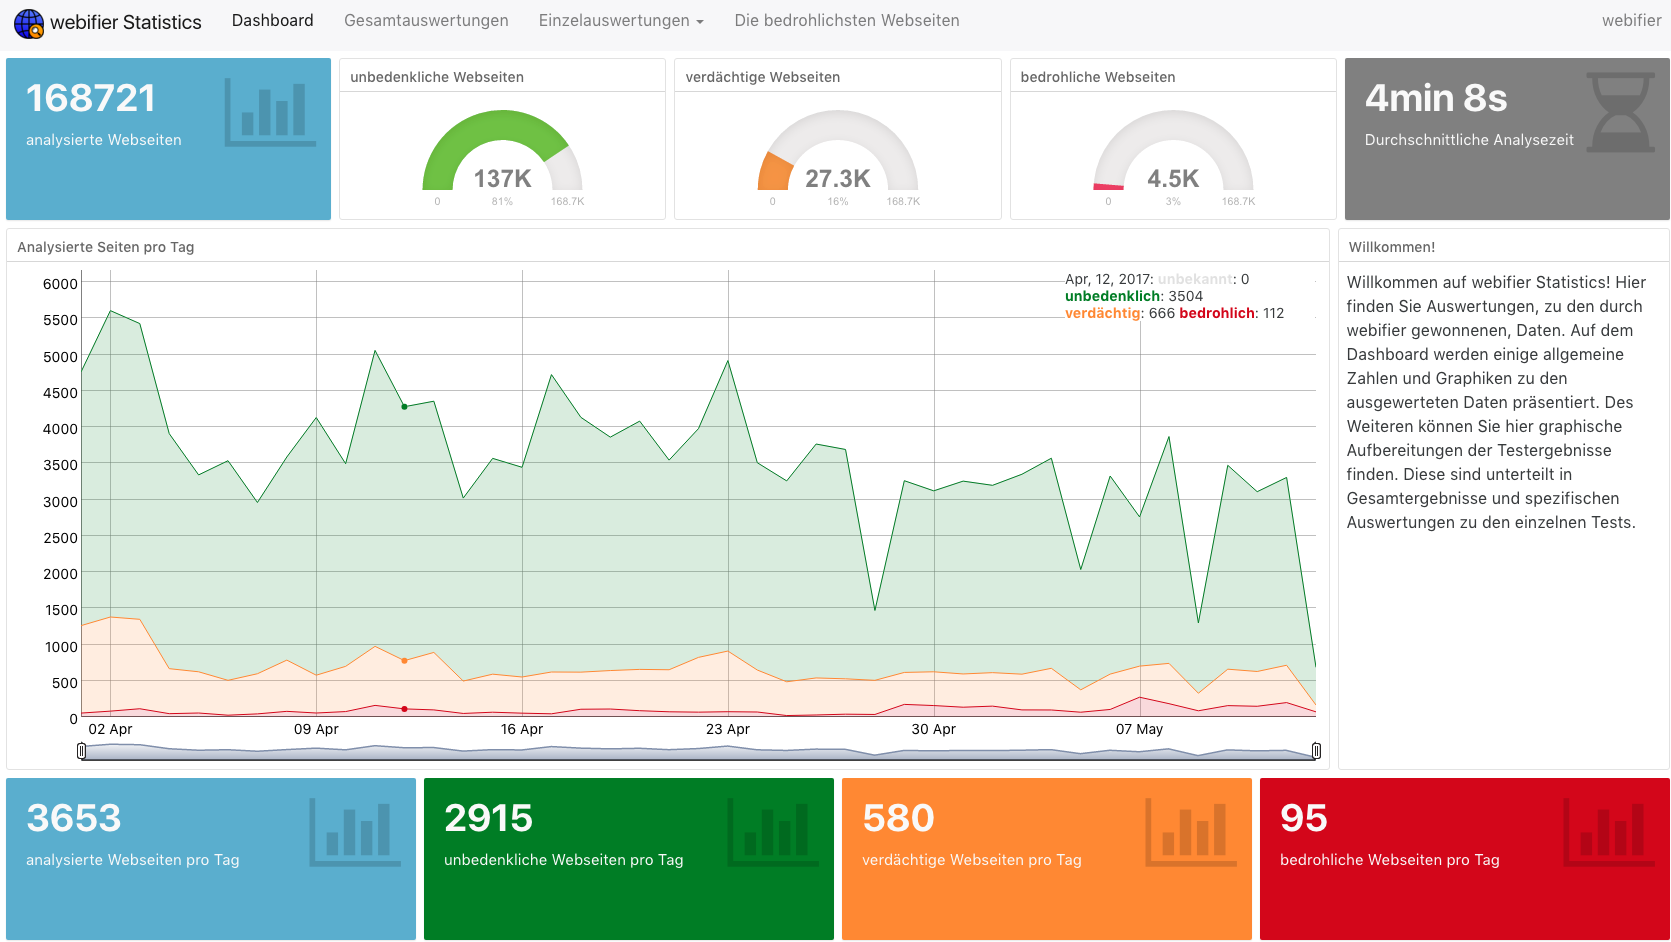
\includegraphics[width=15cm]{images/stats/dashboard}
  \caption[Webifier Statistics Dashboard]{Webifier Statistics Dashboard\protect\footnotemark}
  \label{fig:analyse-dashboard}
\end{figure}
\footnotetext{Die Abbildung befindet sich in besserer Qualität in Anhang \appref{f}.}

An der Oberkante ist eine Navigationsleiste zu finden. Diese wird auf allen Teilseiten angezeigt. Der Nutzer kann hier zwischen den einzelnen Seiten wechseln, hinter dem Reiter \textit{Einzelauswertungen} befindet sich ein Dropdown-Menü zur Auswahl des jeweiligen Testes für den der Nutzer die Statistiken betrachten möchte. In den nachfolgenden Kapiteln wird auf diese Auswertungen genauer eingegangen.

\section{Gesamtauswertungen}
In den Gesamtauswertungen finden sich alle Statistiken, die sich auf die Gesamttests der Webseite beziehen. Ein Gesamttest ist der komplette Durchlauf aller Tests einer Webseite mit aggregiertem Ergebnis. In den folgenden Abschnitten werden die Grafiken beschrieben, die dort zu finden sind.

Der Nutzer hat hier wieder die Möglichkeit über eine zweite Navigationsleiste zwischen den einzelnen Statistiken zu wechseln(siehe Abbildung \ref{fig:tlderkennungen}\todo{dieses Bild gibt es nicht. muss vlt eins zusätzlich eingefügt werden, oder ein bereits eistierendes refernziert werden.} oben). In den folgenden Abbildungen wird dies zugunsten der Übersichtlichkeit nicht angezeigt.

Die erste Statistik(Abbildung \ref{fig:analyse-tlderkennungen}) visualisiert die Anzahl der bedrohlichen und verdächtigen Funde anhand der \ac{TLD}. Zur besseren Übersichtlichkeit werden hier nur Seiten mit bedrohlichem oder verdächtigem Ergebnis gezeigt. Diese werden dann anhand ihrer \ac{TLD} aggregiert und als Balkendiagramm dargestellt. Es werden nur \ac{TLD}, welche mindestens 50 Einträge in der Datenbank haben. Der rote Balken steht für die Anzahl an bedrohlichen Ergebnissen der jeweiligen \ac{TLD} und der gelbe Balken für die verdächtigen Funde. Es fällt auf, dass die \ac{TLD} .com und .de die größten Anteile an beiden Balken haben. Dies ist darauf zurückzuführen, dass diese im \ac{WWW} am weitesten verbreitet sind. Da hier nicht die prozentuale Verteilung der Ergebnisse auf eine \ac{TLD} zu erkennen ist, kann nur Aussage über die Anzahl der Funde in der Datenbank Aussage getroffen werden. Die allgemeine Bedrohlichkeit einer \ac{TLD} kann hieraus nicht abgeleitet werden.
\begin{figure}[H]
  \centering
  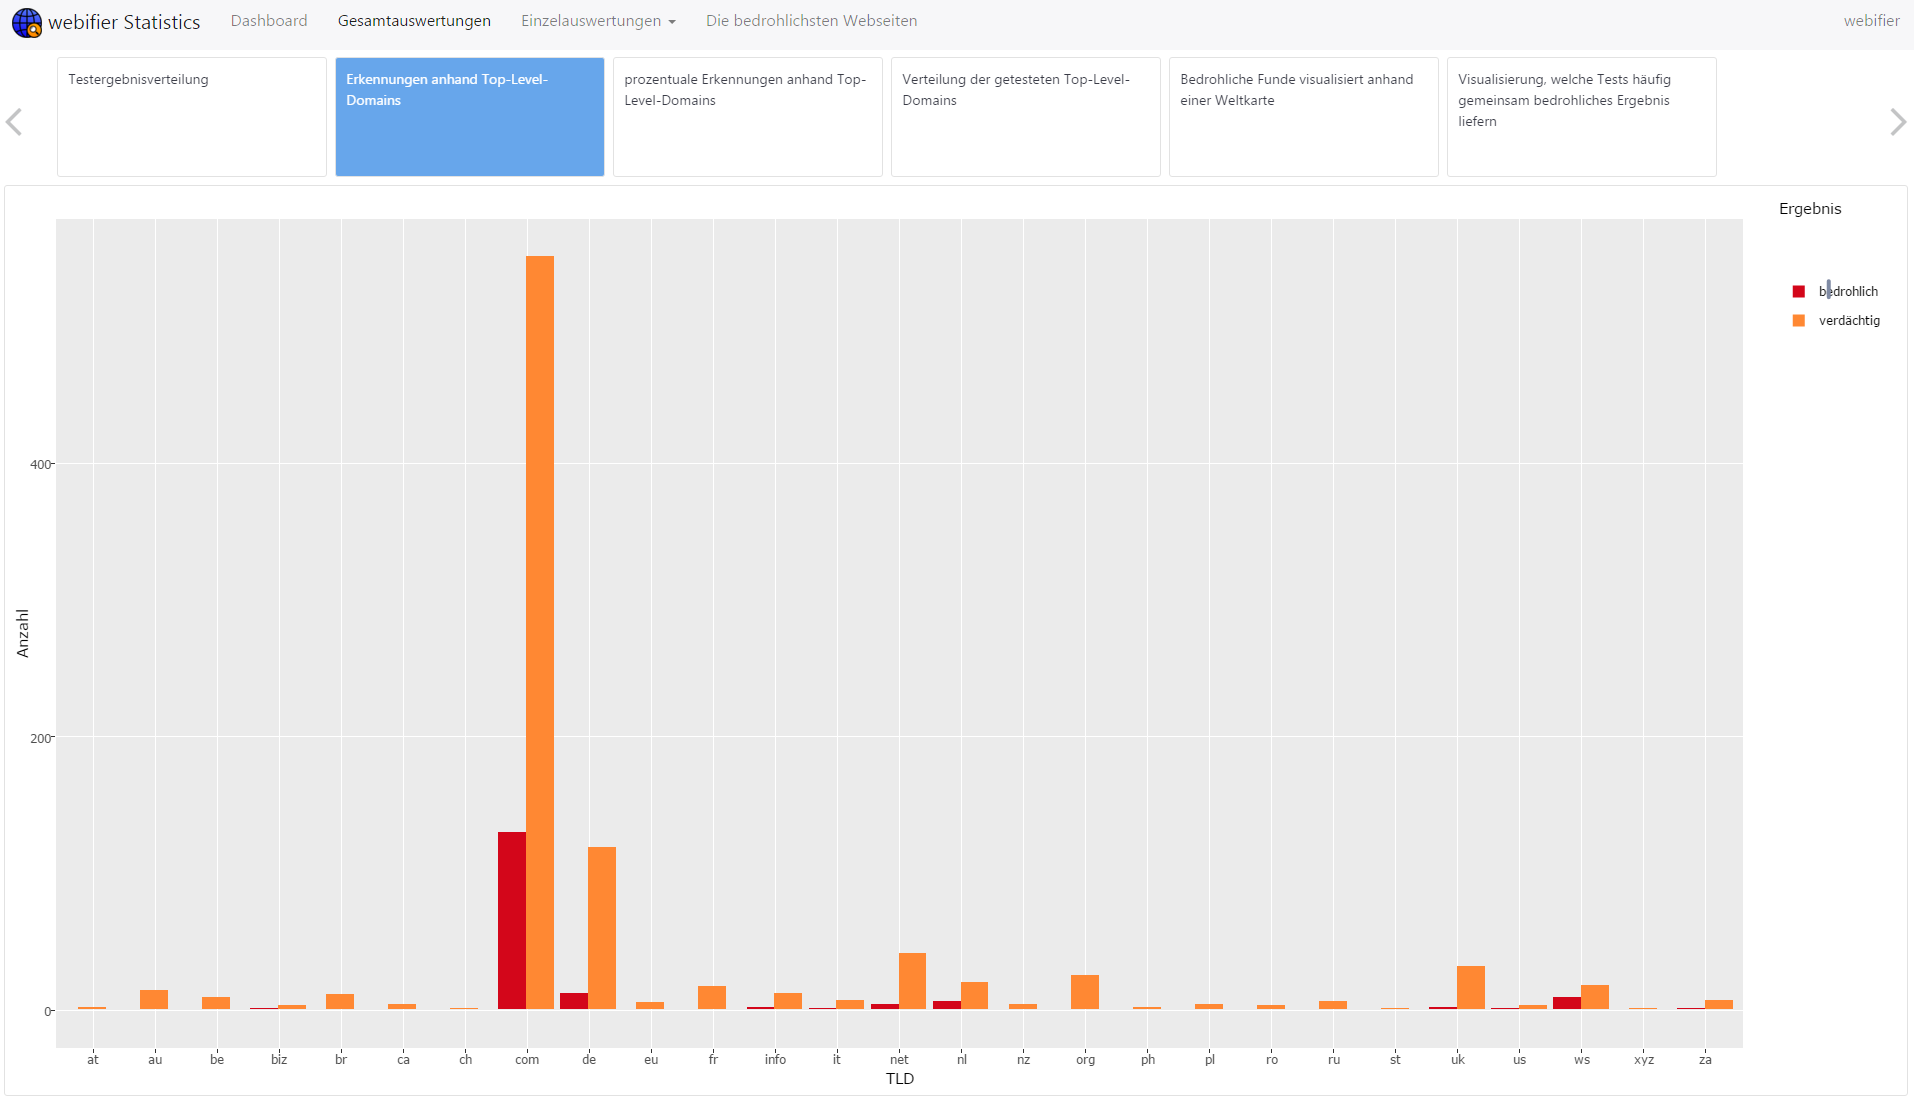
\includegraphics[width=15cm]{images/stats/tlderkennungen}
  \caption[Erkennungen anhand Top-Level-Domains]{Erkennungen anhand Top-Level-Domains\protect\footnotemark}
  \label{fig:analyse-tlderkennungen}
\end{figure}
\footnotetext{Die Abbildung befindet sich in besserer Qualität in Anhang \appref{f}.}

Das, in Abbildung \ref{fig:analyse-tldverteilung} dargestellte, Tortdendiagramm zeigt die Verteilung der getesteten Ergebnisse anhand der \ac{TLD} auf. Auch hier bilden die Top-Level Domains .com (blau - 57.1\%) und .de (orange - 12.5\%) den größten Anteil. Dies bestätigt den Inhalt der vorherigen Grafik, dass diese \ac{TLD},auch für maliziöse Zwecke, sehr verbreitet sind. Sie werden gefolgt von ebenfalls bekannten Adressen wie .net oder .uk.
\begin{figure}[H]
  \centering
  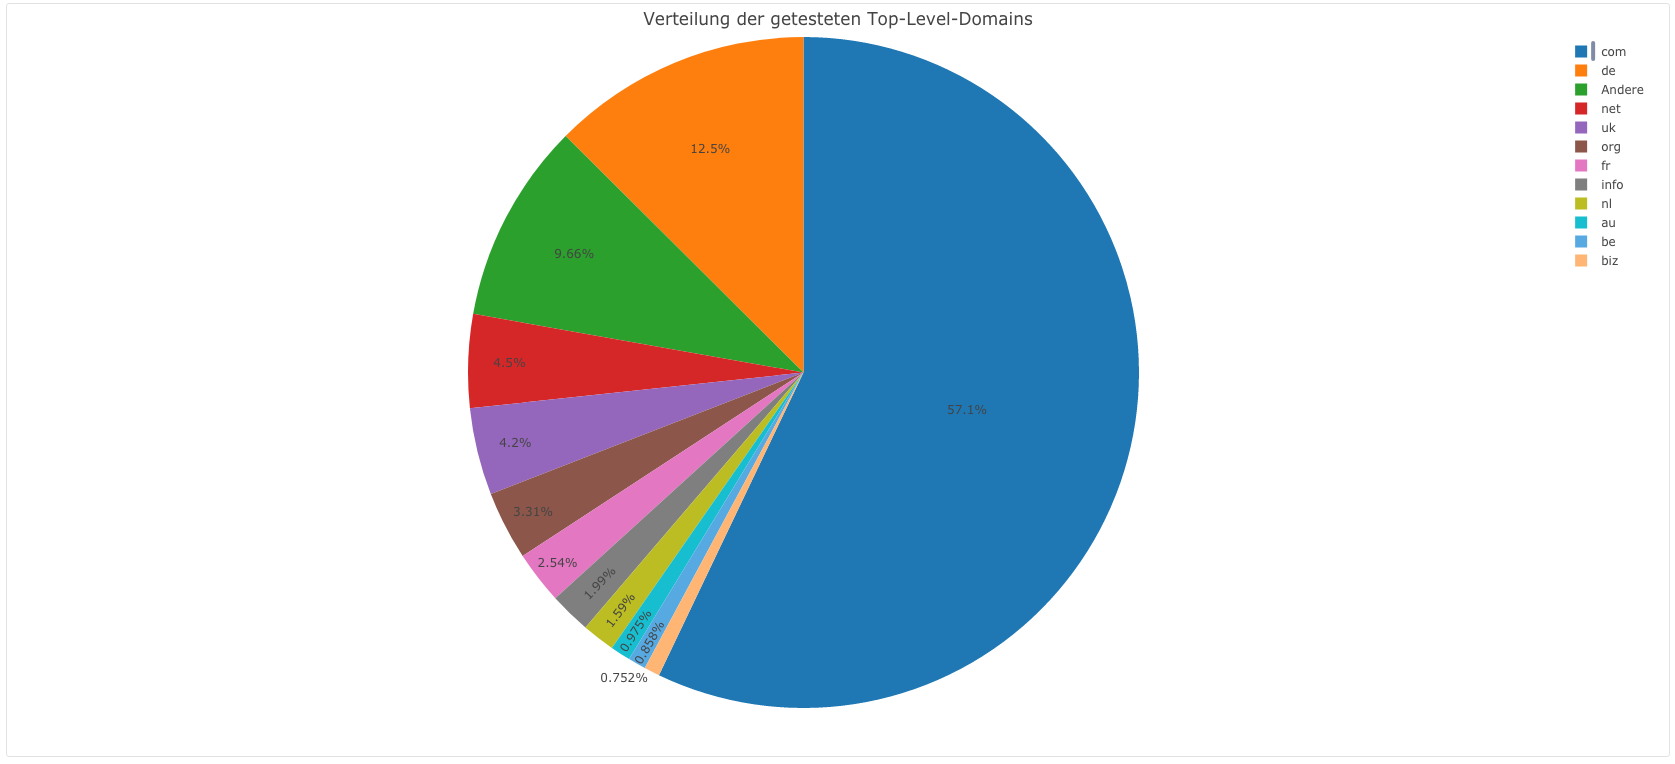
\includegraphics[width=15cm]{images/stats/tldverteilung}
  \caption[Verteilung der getesteten Top-Level-Domains]{Verteilung der getesteten Top-Level-Domains\protect\footnotemark}
  \label{fig:analyse-tldverteilung}
\end{figure}
\footnotetext{Die Abbildung befindet sich in besserer Qualität in Anhang \appref{f}.}

Die Abbildung \ref{fig:analyse-tldprozentual} befasst sich ebenfalls mit den Top-Level Domains. Hier wird die prozentuale Verteilung der Ergebnisse unbedenklich(grün),verdächtig(gelb) und bedrohlich(rot) aufgezeigt. Hier fällt auf, dass die bedrohlichsten \acp{TLD} eher unbekannte sind, wie beispielsweise .pictet oder .sa. Diese beiden kommen auf jeweils 100\% bedrohliche Ergebnisse. Das bedeutet, dass jede Seite mit dieser \ac{TLD} von webifier als bedrohlich erkannt wurde. Die .com-Domain liegt hier im Mittelfeld mit knappen 80\% sauberen Webseiten. Weiterhin ist zu sehen, dass die deutsche \ac{TLD}(.de) in der Liste nicht auftaucht. Dies ist darauf zurückzuführen, dass für diese Auswertung alle Top-Level-Domains mit 100\% sauberen Webseiten vernachlässigt wurden. Wie aus Abbildung \ref{fig:analyse-tlderkennungen} bekannt, wurden aber auch hier bedrohliche Seiten gefunden. Diese sind prozentual gesehen jedoch ein so geringer Anteil, dass sie durch Rundung vernachlässigt wurden.
\begin{figure}[H]
  \centering
  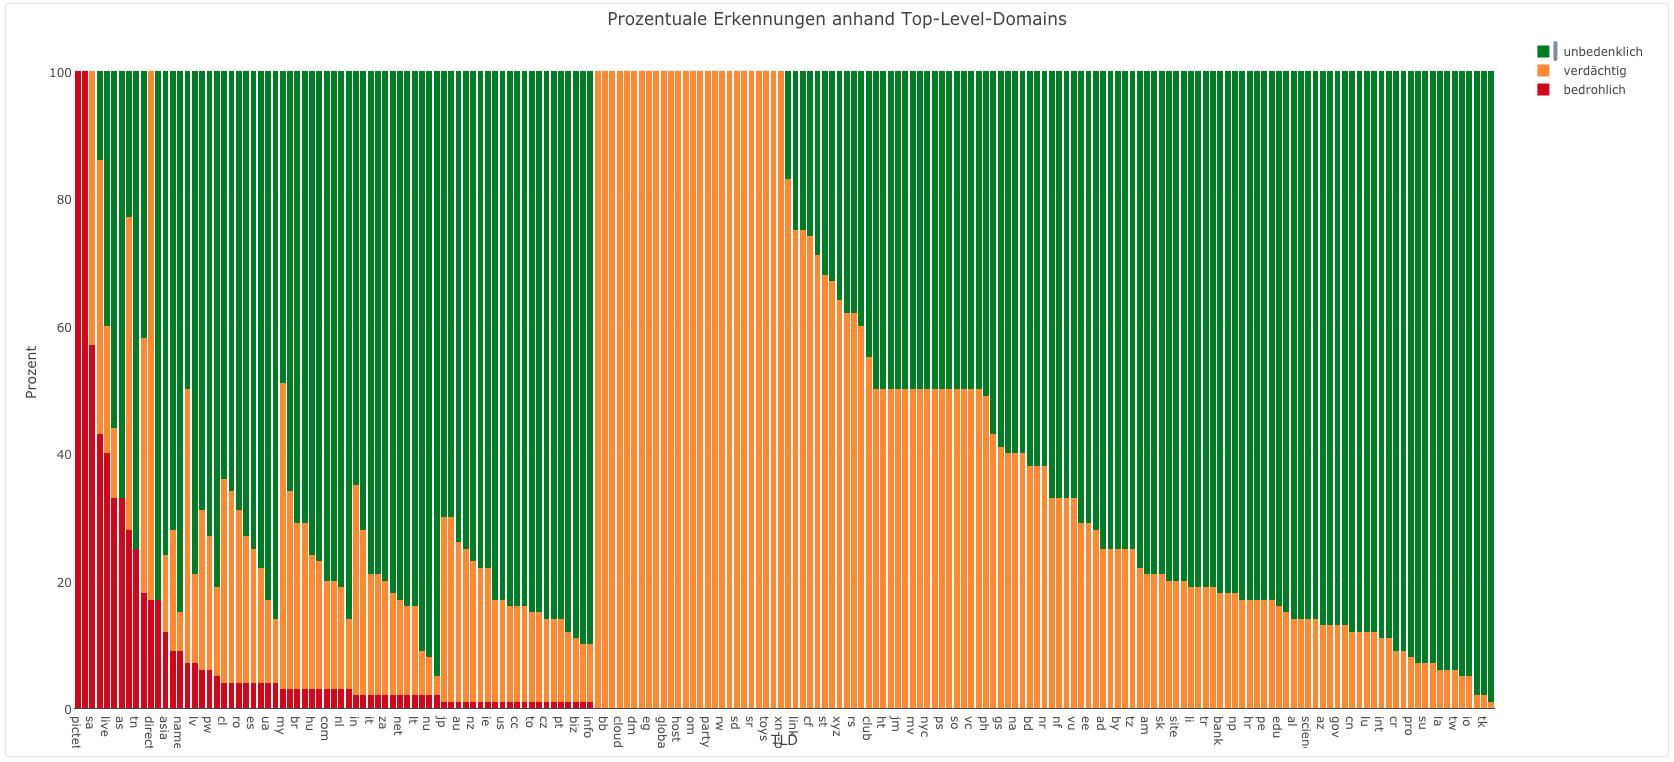
\includegraphics[width=15cm]{images/stats/tldprozentual}
  \caption[prozentuale Erkennungen anhand Top-Level-Domains]{prozentuale Erkennungen anhand Top-Level-Domains\protect\footnotemark}
  \label{fig:analyse-tldprozentual}
\end{figure}
\footnotetext{Die Abbildung befindet sich in besserer Qualität in Anhang \appref{f}.}

Aus den 3 Grafiken zur Verteilung bezogen auf die Top-Level Domains kann erkannt werden, dass bestimmte, eher unbekannte, Top-Level Domains öfter für bedrohliche Zwecke verwendet werden. Jedoch werden auch die bekannten (bspw. .com und .de) Adressen genutzt. Dies lässt sich erklären, dass viele Nutzer im \ac{WWW} bei Webseiten, die auf .de oder .com enden unvorsichtig werden und sich sicher fühlen, da ihnen die \ac{TLD} bekannt ist.

In Abbildung \ref{fig:analyse-weltkarte} wird eine Weltkarte dargestellt, welche sich anhand des Risikofaktors der Länder verfärbt. Der Risikofaktor berechnet sich aus dem durchschnittlichen Ergebniswert aller Ergebnisse des Landes und dies wird mit 100 multipliziert um den prozentualen Wert zu erhalten. Hierbei werden die \ac{TLD} den Ländern zugeordnet. Domains wie .com, welche nicht auf ein bestimmtes Land zurückgeführt werden können, werden in dieser Auswertung vernachlässigt. Länder, für die es keine Zuordnung gab bleiben unausgefüllt.

Es ist zu schnell zu Erkennen, dass die Top-Level Domains für Saudi Arabien(.sa) und Libyen(.ly) den größten Risikofaktor haben. Ein Problem bei dieser Darstellung ist, dass nur die Top-Level Domain der Internetadresse entscheidend ist für die Zuordnung. Für eine genauere Zuordnung müsste man die Lokation anhand der IP-Adresse herausfinden und diese dann den Ländern zuordnen. Denn eine .sa-Domain bedeutet nicht zwangsläufig, dass der Betreiber der Webseite auch in dem jeweiligen Land ansässig ist. Oft wird die Webseite von einem anderen Standort aus betrieben. Einige Betreiber nutzen eine bestimmte Top-Level Domain auch wegen dem Namen. Des Weiteren könnten mit einer Adressierung über IP-Adresse auch jene \ac{TLD} mit einbezogen werden, welche keinem Land zugeordnet sind.

\begin{figure}[H]
  \centering
  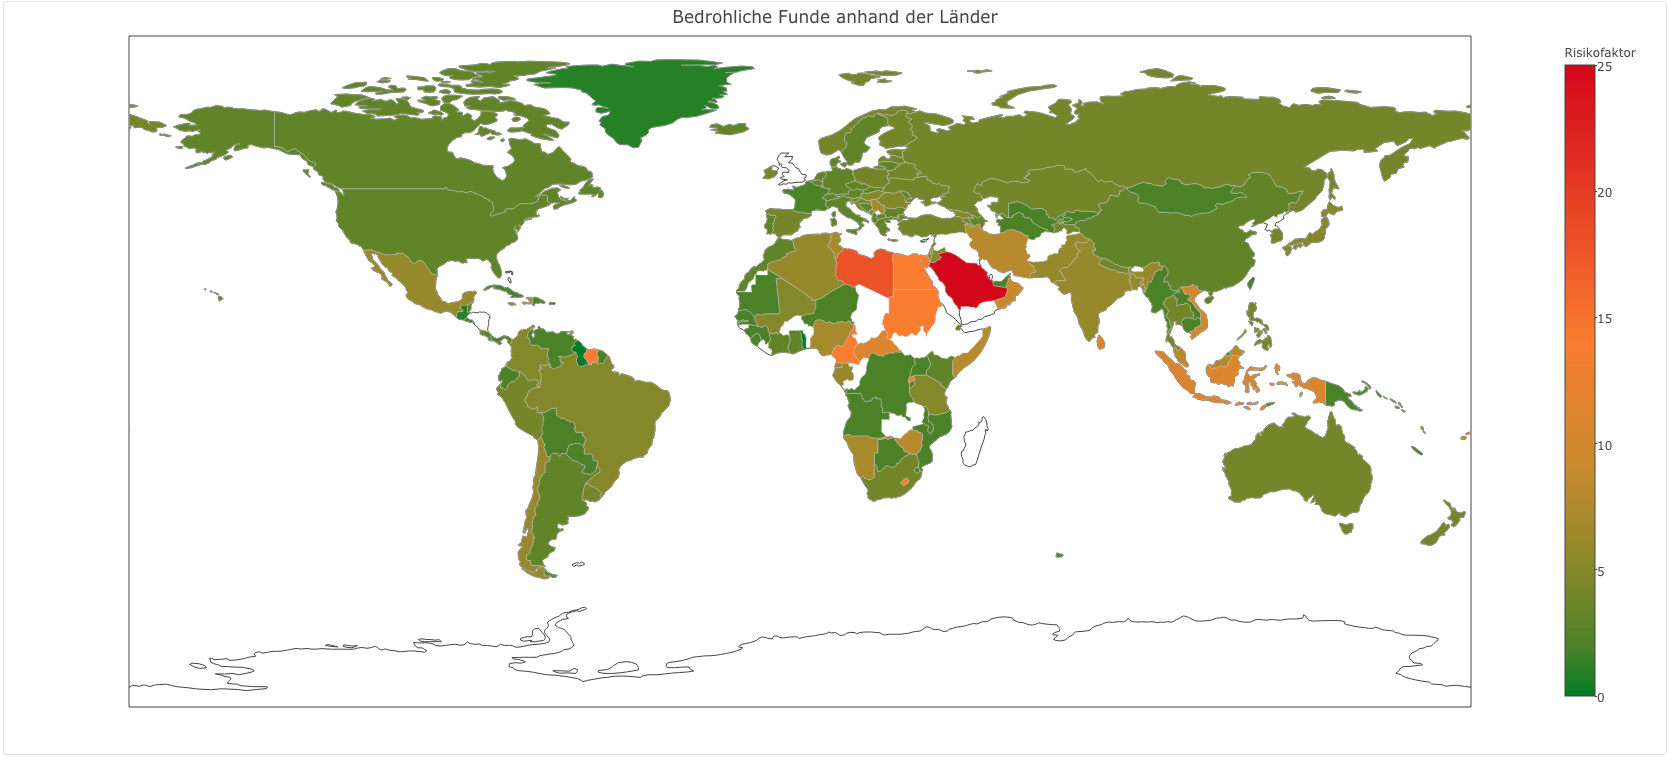
\includegraphics[width=15cm]{images/stats/weltkarte}
  \caption[Bedrohliche Funde visualisiert anhand einer Weltkarte]{Bedrohliche Funde visualisiert anhand einer Weltkarte\protect\footnotemark}
  \label{fig:analyse-weltkarte}
\end{figure}
\footnotetext{Die Abbildung befindet sich in besserer Qualität in Anhang \appref{f}.}

Im folgenden Balkendiagramm (siehe Abbildung \ref{fig:analyse-ergebnisverteilung}) wird die Verteilung der Ergebnisse der einzelnen Tests dargestellt. Für jeden Test werden bis zu 4 Balken für die jeweiligen Ergebnistypen dargestellt.

Hier fällt auf, dass der IP-Scan-Test und der Virusscan-Test nahezu nur saubere Ergebnisse haben. Desweiteren ist zu Erkennen, dass der CertifikateChecker sehr viele verdächtige Seiten gefunden hat. Was dieser Wert aussagt wird im späteren Kapitel über den Test genauer beleuchtet. Eine weitere Beobachtung gibt es bei dem LinkChecker-Test. Dieser hat viele unbekannte Ergebnisse. Dies ist darauf zurückzuführen, dass gerade zu Anfang der Analyse der Datenbestand sehr gering war, so war die Wahrscheinlichkeit, dass eine verlinkte Seite bereits in unseren Daten vorhanden ist sehr gering, somit hat der LinkChecker oft keine Aussage über die Bedrohlichkeit der Seite treffen können.
\begin{figure}[H]
  \centering
  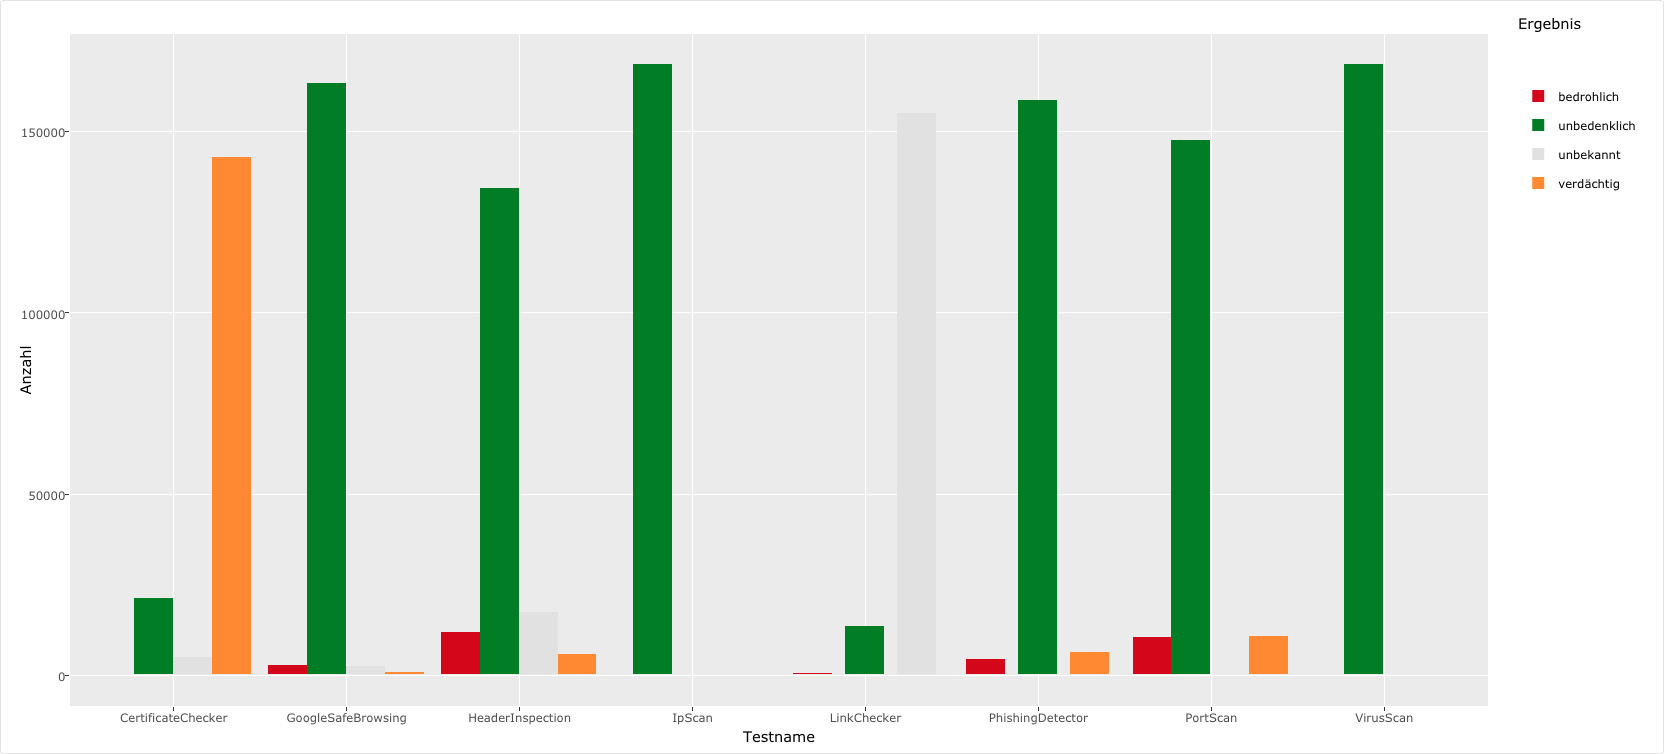
\includegraphics[width=15cm]{images/stats/ergebnisverteilung}
  \caption[Testergebnisverteilung]{Testergebnisverteilung\protect\footnotemark}
  \label{fig:analyse-ergebnisverteilung}
\end{figure}
\footnotetext{Die Abbildung befindet sich in besserer Qualität in Anhang \appref{f}.}

Die nächste Grafik (siehe Abbildung \ref{fig:analyse-testzusammenhaenge}) visualisiert die Zusammenhänge der Tests. Es wird aufgezeigt, welche Tests häufig gemeinsam mit anderen Tests das Ergebnis bedrohlich zur gleichen Webseite liefern. Die Größe der einzelnen Punkte wird über die Anzahl der involvierten Tests bestimmt. Die Anzahl sagt aus wie oft diese Tests die gleiche Seite als bedrohlich klassifiziert haben.

Es ist festzustellen, dass am häufigsten die Tests HeaderInspection und PortScan in der Analyse übereinstimmen. Jedoch lässt eine Anzahl von 1.044 Übereinstimmungen bei knapp 170.000 getesteten und ungefährt 4.500 bedrohlichen Seiten nicht auf einen direkten Zusammenhang schließen. Die weiteren Tests schlagen wenig gemeinsam aus, woraus sich kein Zusammenhang feststellen lässt.

\begin{figure}[H]
  \centering
  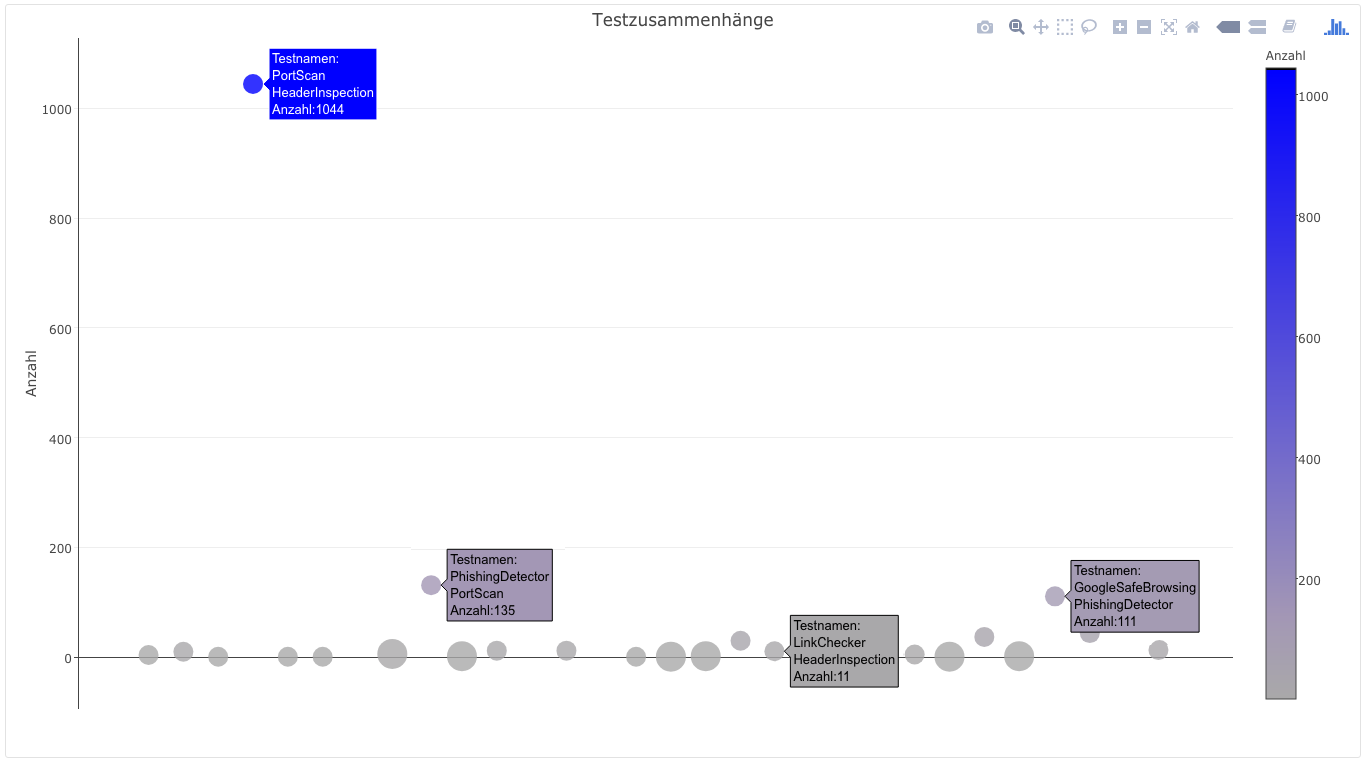
\includegraphics[width=15cm]{images/stats/testzusammenhaenge}
  \caption[Visualisierung der Testzusammenhänge]{Visualisierung der Testzusammenhänge\protect\footnotemark}
  \label{fig:analyse-testzusammenhaenge}
\end{figure}
\footnotetext{Die Abbildung befindet sich in besserer Qualität in Anhang \appref{f}.}

Die Tabelle in Abbildung \ref{fig:analyse-top10} gehört nichtmehr direkt zu den Gesamtauswertungen. Sie ist unter einem eigenen Reiter angesiedelt und dient dazu dem Nutzer zu zeigen, welche Seiten den größten Ergebniswert hatten.
\begin{figure}[H]
  \centering
  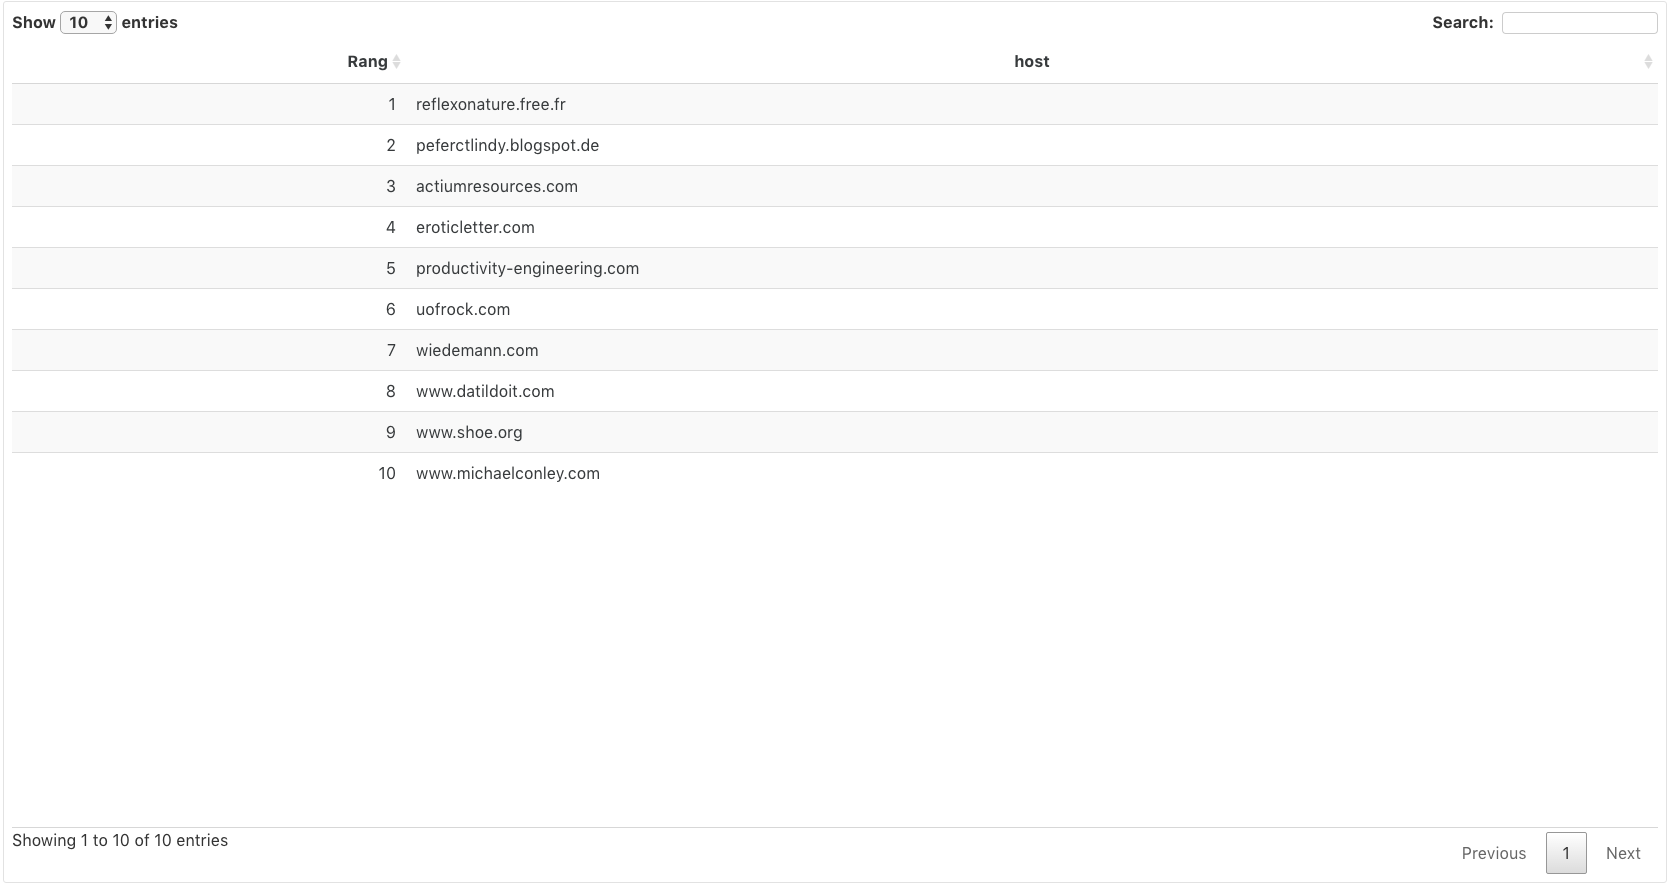
\includegraphics[width=15cm]{images/stats/top10}
  \caption[Top 10: Die bedrohlichsten Webseiten]{Top 10: Die bedrohlichsten Webseiten\protect\footnotemark}
  \label{fig:analyse-top10}
\end{figure}
\footnotetext{Die Abbildung befindet sich in besserer Qualität in Anhang \appref{f}.}

\section{Einzelauswertungen}
In den folgenden Abschnitten werden die Ergebnisse der einzelnen Tests beschrieben und diese bewertet. Abbildung \ref{fig:analyse-headerinspection} zeigt ein Beispiel für eine Seite der Einzelauswertungen eines Testes. Diese Seite ist für die meisten Tests identisch. Deshalb werden im folgenden nur die Kuchendiagramme gezeigt. Für die Überprüfung der Port-Nutzung und dem Virenscan der Webseite sind weitere Kennzahlen vorhanden, welche im jeweiligen Kapitel erläutert werden.

In den Einzelauswertungen sind Kennzahlen zur Anzahl der getesteten Seiten und zur durchschnittlichen Analysezeit. Darunter befindet sich ein Kuchendiagramm, welches die prozentuale Verteilung der Testergebnisse visualisiert.
\begin{figure}[H]
  \centering
  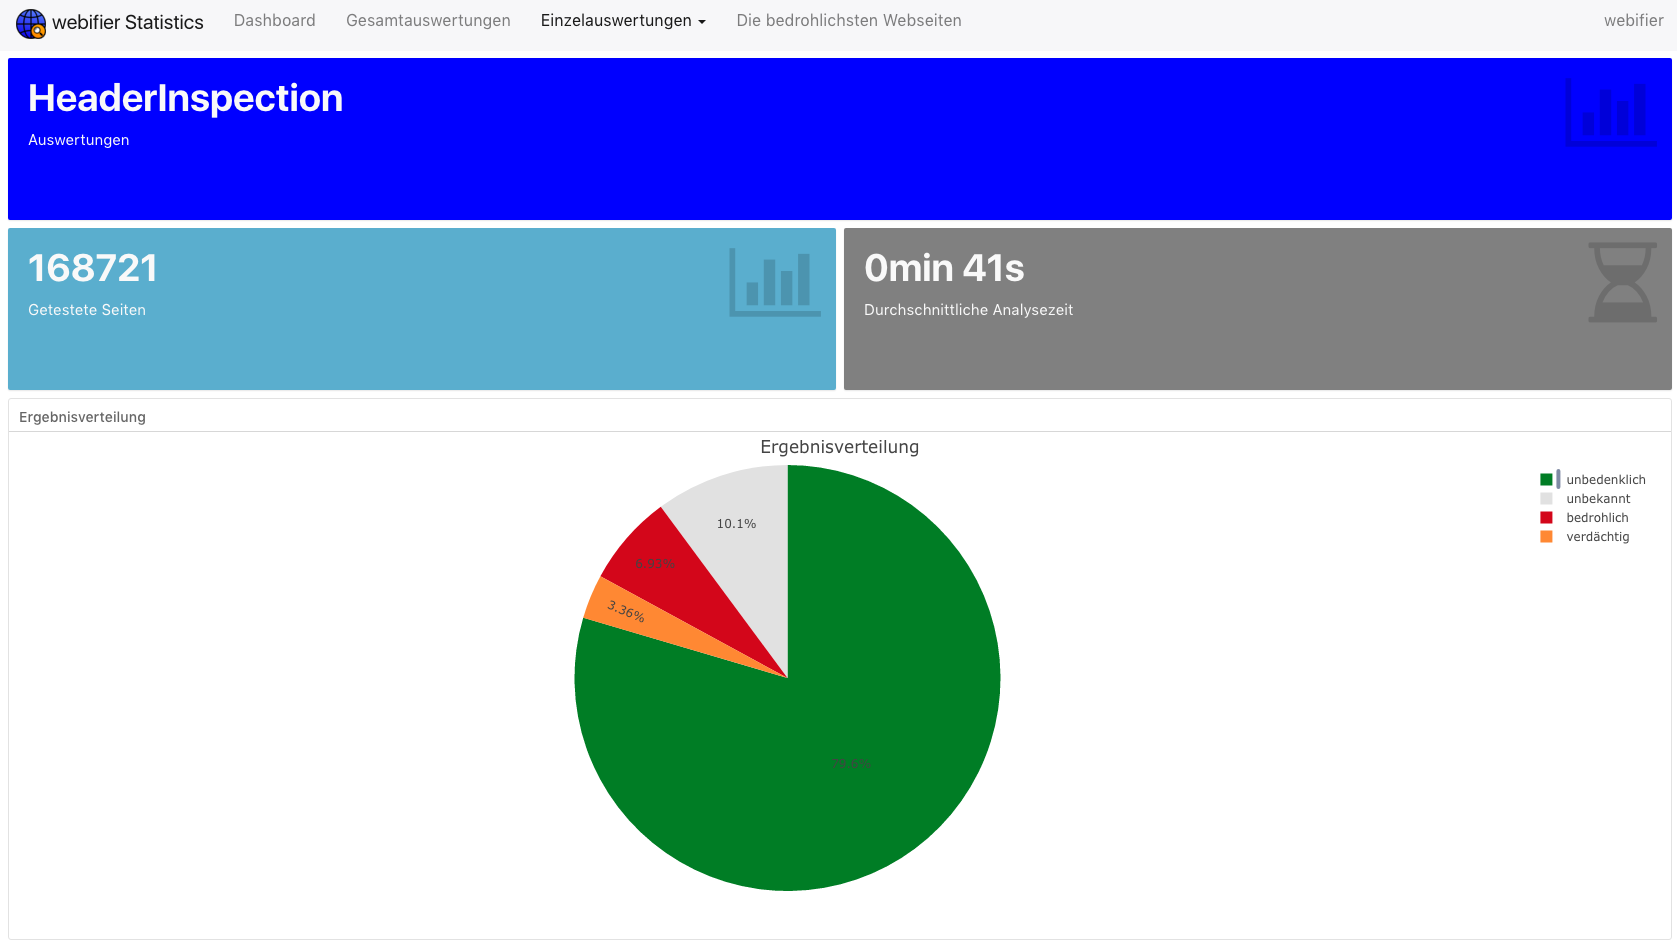
\includegraphics[width=15cm]{images/stats/headerinspection}
  \caption[Einzelauswertung: Vergleich in verschiedenen Browsern]{Einzelauswertung: Vergleich in verschiedenen Browsern\protect\footnotemark}
  \label{fig:analyse-headerinspection}
\end{figure}
\footnotetext{Die Abbildung befindet sich in besserer Qualität in Anhang \appref{f}.}

\subsection{Virenscan der Webseite}
\begin{figure}[H]
  \centering
  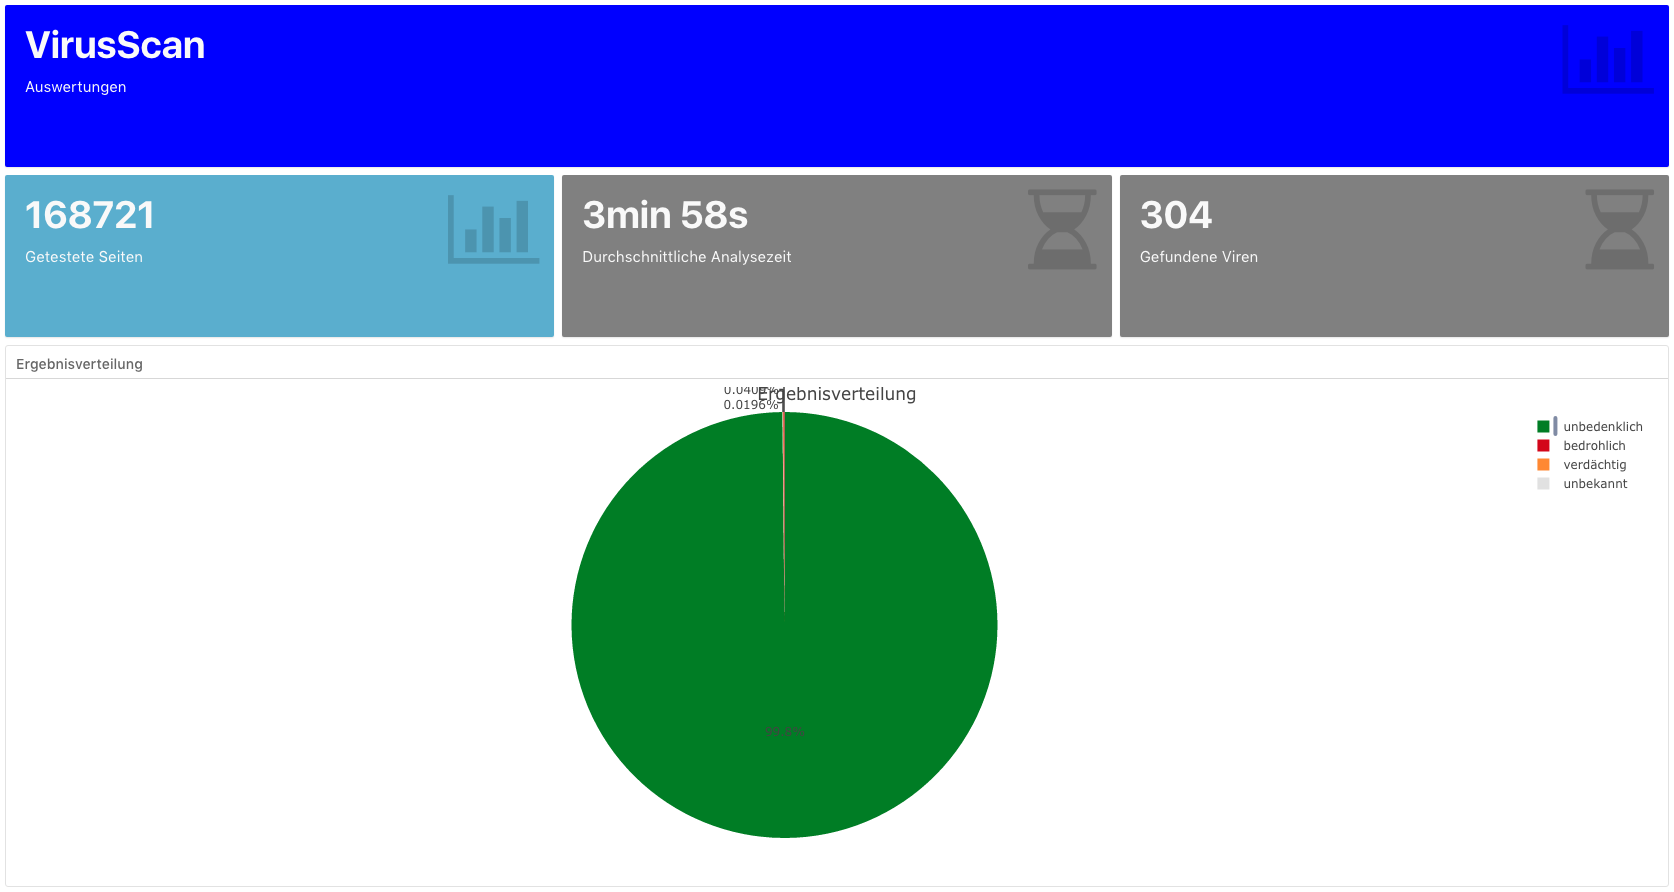
\includegraphics[width=15cm]{images/stats/virusscan}
  \caption[Einzelauswertung: Virenscan der Webseite]{Einzelauswertung: Virenscan der Webseite\protect\footnotemark}
  \label{fig:analyse-virusscan}
\end{figure}
\footnotetext{Die Abbildung befindet sich in besserer Qualität in Anhang \appref{f}.}

Wie das Kreisdiagram in Abbildung \ref{fig:analyse-virusscan} zeigt enthielten nur etwa 0,2\% der überprüften Domains Malware. Dennoch wurden insgesamt über 300 Schadprogramme entdeckt, weshalb die Verbreitung von Viren, Würmern, Trojanern und anderer Malware nach wie vor auch über Webseiten im Internet geschieht. Aus diesem Grund sollte besonders bei zwilichtigen Webangeboten Vorsicht geboten sein.

\subsection{Vergleich in verschiedenen Browsern}
\begin{figure}[H]
  \centering
  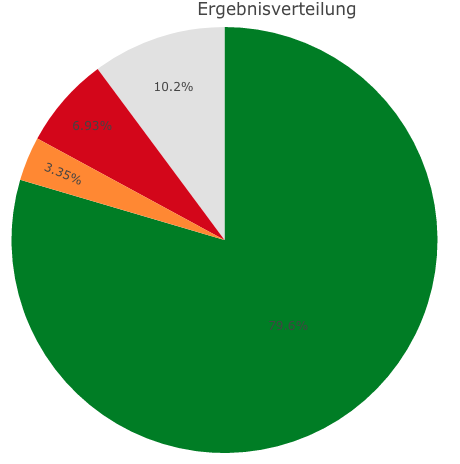
\includegraphics[width=5cm]{images/stats/diaheaderinspection}
  \caption{Vergleich in verschiedenen Browsern - Testergebnisverteilung}
  \label{fig:analyse-diaheaderinspection}
\end{figure}

Im \textit{Vergeleich in verschiedenen Browsern} wurde die größte Quote an bösartigen Webseiten
erreicht. Laut Abbildung \ref{fig:analyse-diaheaderinspection} wurden durch diesen Test 6,93\% der
Webseiten als \textit{MALICIOUS} eingestuft. Das Kriterium für dieses Ergebnis ist eine maximale
Abweichung von 500 Zeichen zwischen den erhaltenen Antworten der diversen Browser. In diese
Größenordnung ist zu groß für Zeitangaben oder andere Unterschiede, die durch den Zeitpunkt des
Aufrufs entstehen können. Leider kann durch die bloße Angabe der Zeichenunterschiedslänge keine
qualitative Aussage über den Hintergrund dieser Verschiedenheit gemacht werden. Besser wäre es,
wenn man die unterschiedlichsten Antworten auf JavaScript und Links zu anderen Webressourcen untersuchen würde.

\subsection{Überprüfung der Port-Nutzung}

\begin{figure}[H]
  \centering
  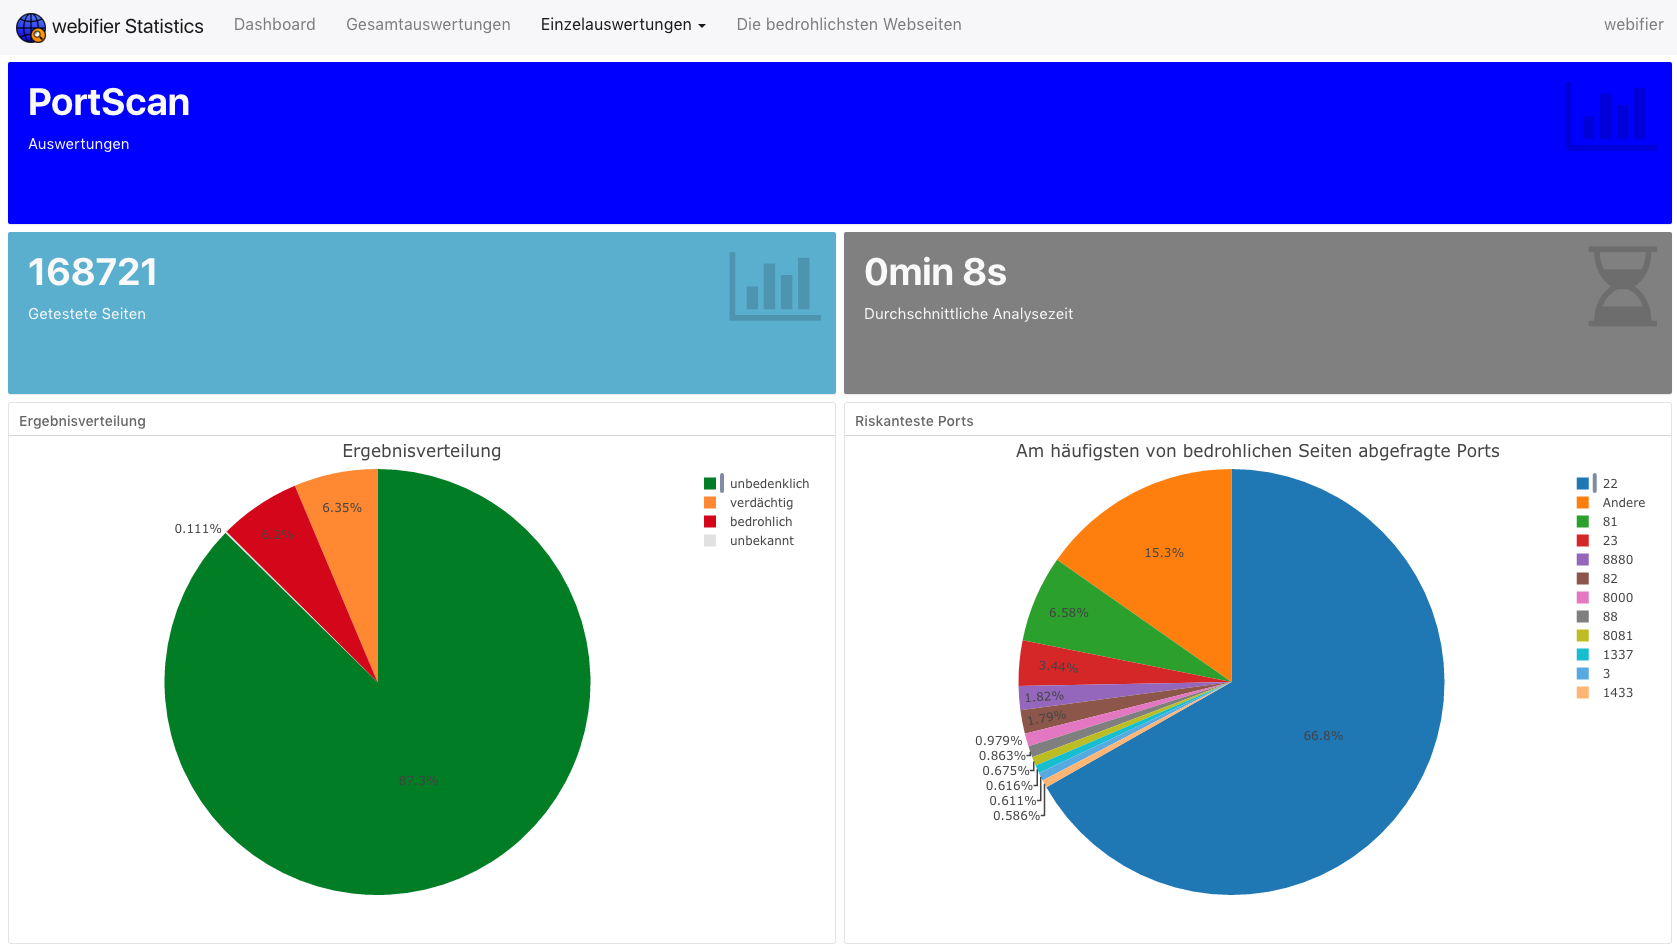
\includegraphics[width=15cm]{images/stats/portscan}
  \caption[Einzelauswertung: Überprüfung der Port-Nutzung]{Einzelauswertung: Überprüfung der Port-Nutzung\protect\footnotemark}
  \label{fig:analyse-portscan}
\end{figure}
\footnotetext{Die Abbildung befindet sich in besserer Qualität in Anhang \appref{f}.}

Abbildung \ref{fig:analyse-portscan} zeigt die Ergebnisse des Testes zur Überprüfung der
Portnutzung.
Hier ist festzustellen, dass Portscanning ein eher wenig genutztes Mittel ist, da 87.3\% der Webseiten unbedenklich sind. Zudem läuft der Test mit gerade einmal 0.111\% unbekannten Ergebnissen sehr stabil, denn das Ergebnis unbekannt kann hier nur entstehen indem der Test abstürzt.

Neben der Ergebnisverteilung gibt es hier noch ein weiteres Kuchendiagramm zur Visualisierung der abgefragten Ports. Hier werden alle Ports anhand der Häufigkeit ihrer Abfrage aufgelistet. Hier ist erkennbar, dass Port 22, mit 66.8\%, der am häufigsten abgefragte Port ist. Da dies der für SSH standardisierte Port ist, kann dies ein Indiz sein, dass Webseiten versuchen sich über SSH Zugriff verschaffen wollen.

\subsection{Überprüfung der IP-Nutzung}

\begin{figure}[H]
  \centering
  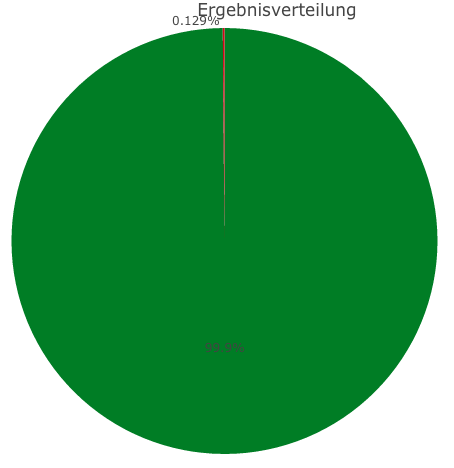
\includegraphics[width=5cm]{images/stats/diaipscan}
  \caption{Überprüfung der IP-Nutzung - Testergebnisverteilung}
  \label{fig:analyse-diaipscan}
\end{figure}

Der Test zur Überprüfung der IP-Nutzung hat keinerlei bedrohliche oder verdächtige Webseiten erkannt(siehe Abbildung \ref{fig:analyse-diaipscan}). Wie auch der Test zu Überprüfung der Port-Nutzung läuft dieser Test sehr stabil mit 0.129\% unbekannten Ergebnissen. Da beide Tests fast identisch implementiert sind wird ein Fehler in der Umsetzung ausgeschlossen.

\subsection{Prüfung aller verlinkten Seiten}
\begin{figure}[H]
  \centering
  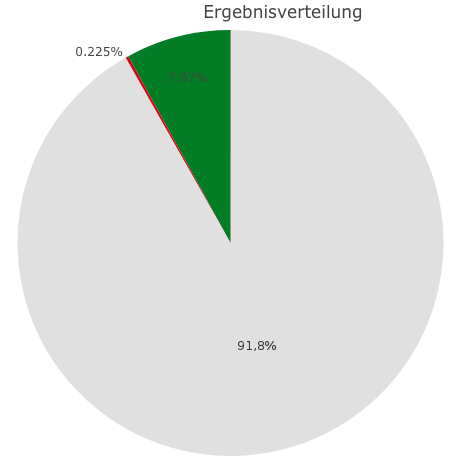
\includegraphics[width=5cm]{images/stats/dialinkchecker}
  \caption{Prüfung aller verlinkten Seiten - Testergebnisverteilung}
  \label{fig:analyse-dialinkchecker}
\end{figure}

Während der Analysephase wurden vom Test \textit{Prüfung aller verlinkten Seiten} ganze 91,8\% der
Seiten als \textit{UNDEFINED} klassifiziert (Abbildung \ref{fig:analyse-dialinkchecker}).
Dieses Ergebnis ist nicht allzu überraschend, da in diesem, Test gegen die systeminterne Datenbank getestet wird.
Diese war zu Beginn der Analysephase noch komplett leer, sodass \textbf{alle} Tests \textit{UNDEFINED} ergaben.
Im laufe der Analyse wurde die Datenbank voller, was man an den 7,97\% sauberen und immerhin
0,225\% maliziösen Einträgen erkennen kann.

\subsection{Google Safe Browsing}
\begin{figure}[H]
  \centering
  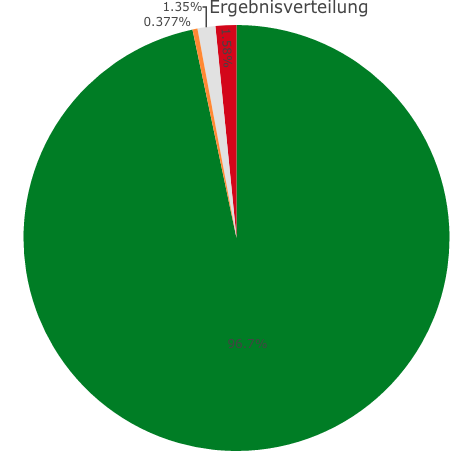
\includegraphics[width=5cm]{images/stats/diagoogle}
  \caption{Google Safe Browsing - Testergebnisverteilung}
  \label{fig:analyse-diagoogle}
\end{figure}

Wie in Abbildung \ref{fig:analyse-diagoogle} zu sehen ist, wurden lediglich 1,58\% der
getesteten Seiten als \textit{MALICIOUS} und ganze 96,7\% als \textit{CLEAN} eingestuft.
Leider kann nicht davon ausgegangen werden, dass alle Seiten im \textit{CLEAN}-Bereich tatsächlich unbedenklich sind.
Denn es ist sehr wahrscheinlich, dass Google viele der getesteten Seiten noch nicht in ihrer Datenbank abgespeichert hat.
Besser wäre es, wenn der Google Safe Browsing Service eine Art \textit{CLEAN}-Ergebnis für bekannte, nichtmaliziöse Webseiten ausgeben würde, statt einfach kein Ergebnis zurückzuliefern. 

\subsection{Überprüfung des SSL-Zertifikats}
\begin{figure}[H]
  \centering
  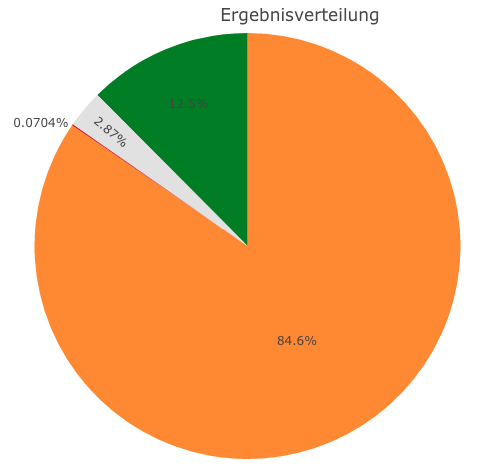
\includegraphics[width=5cm]{images/stats/diacertificate}
  \caption{Überprüfung des SSL-Zertifikats - Testergebnisverteilung}
  \label{fig:analyse-diacertificate}
\end{figure}

Sehr positiv an diesem Test ist wohl, dass kaum fehlerhafte Zertifikate gefunden wurden, wie
Abbildung \ref{fig:analyse-diacertificate} zeigt. Beunruhigend ist hingegend das fast 84\% aller getesteten Webseiten überhaupt kein Zertifikat verwenden. Zumal der Erwerb eines Zertifikates auch finanziell keine Probleme mehr darstellt, da es wie an anderer Stelle bereits erwähnt Vergabestellen gibt, welche kostenlose Zertifikate ausstellen.

\subsection{Erkennung von Phishing}
\begin{figure}[H]
  \centering
  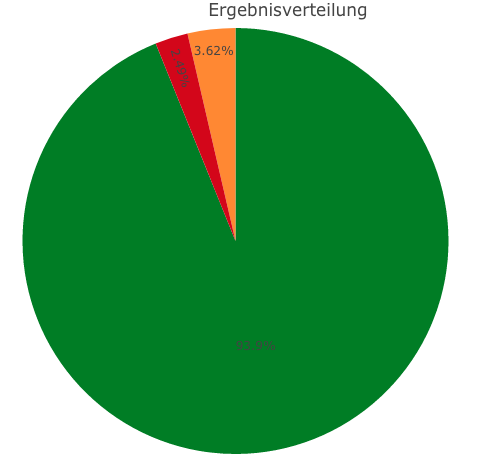
\includegraphics[width=5cm]{images/stats/diaphishing}
  \caption{Erkennung von Phishing - Testergebnisverteilung}
  \label{fig:analyse-diaphishing}
\end{figure}

Etwa 6\% der überprüften Seiten wurden als Phishingseiten eingestuft. Absolut betrachtet wurden ca. 10.000 Phishingseiten von webifier gefunden. Allerdings sollten diese Werte aufgrund der Einfachheit des mit Vorsicht betrachtet werden, da deshalb auch einige Webseiten fehlerhaft klassifiziert wurden. Wichtig zu beachten ist außerdem das viele Phishingseiten nur wenige Minuten oder Stunden existieren, weshalb der Erkennungszeitraum auch entsprechend gering ist.

\section{Bewertung der Ergebnisse}
Zur Bewertung der Ergebnisse müssen alle Tests betrachtet werden. Verwunderlich ist hierbei, die geringe Anzahl an gefundener Viren. In den Grundlagen wurde analysiert, dass die Verbreitung von Malware in Deutschland stark zugenommen hat(siehe Abbildung \ref{fig:malware}), jedoch die Ergebnisse von webifier auf eine geringe Malware-Verbreitung schließen lassen. Dies kann beweisen, dass Malware sich nicht durch maliziöse Webseiten verbreitet. Ein weiterer Grund für dieses Ergebnis ist, dass eventuelle versteckte Downloads auf den entsprechenden Seiten nicht mit analysiert wurden.

Des Weiteren ist überraschend, dass knapp 84\% der getesteten Webseiten kein Zertifikat nutzen, ob wohl dies heutzutage ohne finanziellen Aufwand erhältlich ist.

In der Verteilung der getesteten Top-Level Domains lassen sich Unterschiede bezüglich der weltweiten
Anzahl an genutzten Top-Level
Domains\footnote{\url{https://w3techs.com/technologies/overview/top_level_domain/all}} erkennen. Der
hauptsächliche Unterschied liegt in der Nutzung der russischen Domain. Diese liegt weltweit auf Platz 2 der am häufigsten genutzten Domainendungen. In den von webifier getesteten Seiten taucht diese Endung allerdings sehr selten auf. Die .com-Domain ist in der Analyse von webifier ähnlich stark vertreten wie in der weltweiten Verteilung.

Zur Bewertung der Ergebnisse müsste noch die Güte der genutzten Blacklists überprüft werden. Da dies nicht einfach ist würde eine größer angelegte Suche mit weiteren Webseiten die Ergebnisse aussagekräftiger machen. Im hier beschränkten Zeitraum von 1 Monat zur Analyse konnten bisher nur knapp 170.000 Webseiten analysiert werden. Dies stellt nur einen kleinen Bruchteil der im World Wide Web verfügbaren Webseiten dar. Eine länger angelegte Suche würde die Ergebnisse aussagekräftiger machen.

Bei Betrachtung der Tests zur Überprüfung der Port- \& IP-Nutzung ist festzustellen, dass die Verbreitung dieser Angriffstypen eher gering ausfällt. Dies ist nicht verwunderlich, da diese Art von Angriffstypen meist für gezielte Angriffe genutzt werden. Der Angreifer hat meist ein bestimmtes Ziel im Auge und versucht mittels IP- \& Port-Scanning Schwachstellen im System des Opfers zu finden, über welche dann ein Hacker-Angriff gestartet werden kann. Die Nutzung dieser Scans auf Webseiten um sämtliche Nutzer auszuspähen ist daher wie erwartet gering.

Zur Bewertung der Ergebnisse lässt sich abschließend sagen, dass die Anzahl an gefundenen Bedrohungen geringer als erwartet ist, dies sich aber auch auf die begrenzte Analysezeit zurückführen lässt. Im folgenden Kapitel wird auf die Zukunft von webifier eingegangen, wie die Plattform erweitert und verbessert werden kann um weitere Auswertungen zu starten.
